\documentclass[11pt]{article}
\input{/Users/markwang/.preamble}
\begin{document}


\section*{Problem 1}

\begin{enumerate}
    \item 
    Given an algorithm taking inputs
    \begin{enumerate}
        \item $G = (V,E)$ a connected, undirected graph 
        \item $w: E\to \mathbb{Z}^+$ a weight function 
        \item $T \subseteq E$, a MST of $G$
        \item $e_1 = \{u,v\} \not\in E$, an edge no in $G$ 
        \item $w_1 \in \mathbb{Z}^+$, a weight for $e_1$
    \end{enumerate}
    and outputs a MST $T_1$ for $G_1 = (V, E\cup \{ e_1 \})$ with $w(e_1) = w_1$. For full marks, your algorithm must be more efficient than computing a MST for $G_1$ from scratch. Justify that this is the case by analysing your algorithm’s worst-case running time. Finally, write a detailed proof that your algorithm is correct. 


    \begin{solution}
        \textbf{Algorithm}
        \begin{enumerate}
            \item Let $G_1 = (V, E\cup \{ e_1 \})$, let $e_1 = (s,t)$ for some $s,t\in V$ 
            \item Find the unique simple cycle $c$ in $G_1$. Starting from $s$ (or $t$, the choice is arbitrary), run DFS on $G_1$ with slight modification. When looking at vertex $u\in V$, Check if $v.color$ is $GRAY$. Break from DFS if true, otherwise continue DFS. 
            \item Find the largest weight edge $e_2$ in the cycle. Iterate through $G_1.E$, find $e_2 = (u,v)\in G_1.E$ such that $u.color$ and $v.color$ are both $GRAY$ (in the cycle) and $w(u,v)$ is maximum of all edges with $GRAY$ vertices (max weighted edge). 
            \item Return MST $T_1 = T \cup \{ e_1 \} \setminus \{e_2 \}$ 
        \end{enumerate}
        \textbf{Analysis} 
        \begin{enumerate}
            \item Since we are adding a constant time check at every while iteration and DFS itself has a run time of $O(V+E)$, the part of algorithm for finding a cycle (modified DFS) has a worst case running time of $O(V+E)$
            \item The loop over all vertices to locate the maximum weight edge runs for $|E|$ iterations, each time doing a constant time operation. hence has a worst case running time of $O(E)$
            \item Altogether the algorithm runs for $O(V+E)$, which is more efficient by computing MST from ground up which takes $O(E\lg V)$
        \end{enumerate}




        \begin{algorithm}[H]
            \SetKwFunction{mst}{Find-MST-1}
            \SetKwFunction{pop}{Stack-Pop}
            \SetKwFunction{top}{Stack-Top}
            \SetKwFunction{insert}{Stack-Insert}
            \SetKwFunction{dfs}{DFS-Visit}  
            \SetKwFunction{break}{Exit-DFS}  

            \Fn{\dfs$(G,u)$}{
                $u.color \leftarrow GRAY$\\
                \For{$v\in G_1.Adj[u]$}{
                    \If{$v.color$ is $GRAY$}{
                        \break
                    }
                    \If{$v.color$ is $WHITE$}{
                        $\dfs(G, v)$
                    }
                }
                $u.color \leftarrow BLACK$\\
            }

            \Fn{\mst$(G, w, T, e_1, w_1)$}{
                $G_1 \leftarrow (V, E = E\cup \{ e_1\})$ with $w:E\to\R$ and $w(e_1) = w_1$  \\
                $(s, t) \leftarrow e_1$\\

                \For{$v\in V$}{
                    $v.color \leftarrow WHITE$\\
                }
                $\dfs(G_1, s)$\\
                $max_w \leftarrow 0$ \\
                $e_2 \leftarrow NIL$\\
                \For{$(u,v) \in G_1.E$}{
                    \If{$u.color = GRAY$ and $v.color = GRAY$ and $w(u,v) > max_w$}{
                        $max_w \leftarrow w(u,v)$\\
                        $e_2 \leftarrow (u,v)$\\
                    }
                }
                $T_1 \leftarrow T \cup \{ e_1 \} \setminus \{e_2 \}$
                \Return{$T_1$}
            }
        \end{algorithm}

        \begin{lemma*}
            The graph $G_1 =(V, E = E\cup \{ e_1\})$ has a unique simple cycle $c$, and $e_1$ is in $c$
            \begin{proof}
                Let $T \subseteq E$, and $e_1 = (s,t)$. Since $T$ is MST, $s$ is reachable from $t$, i.e. exists a path $p$ such that $t \overset{p}{\leadsto} s$. Consider $E_1 = E \cup \{ e_1\}$, we have $c = s\to t \overset{p}{\leadsto} s = \langle v_0 = s, \cdots, v_k = s \rangle$. Therefore $e_1$ is in $c$. Now we prove $c$ is unique. This is equivalent to proving that $p$ is unique, since if adding $e_1$ to $E$ produces more than 1 cycle, then there must exists $p'$ such that $p' \neq p$. This is not possible since $s \overset{p}{\leadsto} t \overset{p'}{\leadsto} s$ forms a cycle, which is not possible in MST $T$. Also, $c$ is simple because $T$ is simple. 
            \end{proof}
        \end{lemma*}

        \textbf{Proof of correctness} 
        \begin{proposition*}
            The output $T_1$ is a MST for $G_1 =(V, E = E\cup \{ e_1\})$
            \begin{proof}
                By correctness of DFS, when we first explored $(u,v)$, if $v.color$ is $GRAY$, then $(u,v)$ is a back edge, indicating we have found a cycle $c$ in the graph. By the previous lemma and the fact that we started from $s$ where $e_1 = (s,t)$, we will always find such a cycle (i.e. discover $t$ such that $s\in G_1.Adj[t]$ and $s.color$ is $GRAY$). When \textsc{Exit-DFS} is called, the vertices $v\in V$ such that $v.color$ is $GRAY$ represents vertices constituting the cycle $c$. The claim holds since by the time \textsc{Exit-DFS} is called, all ancestors of $t$ has yet to finish (i.e. setting their color to $BLACK$). The subsequent loop over $G_1.E$ finds the maximum weighted edge $e_2$ in the cycle $c$. By the cycle property of MST, $e_2$ cannot be included in any MST of $G_1$. Now consider the return value $T_1 = T \cup \{ e_1 \} \setminus \{e_2 \}$. Now we prove $T_1$ is a MST of $G_1$. Consider $A = T \setminus \{ e_2 \}$, note $A$ breaks into 2 connected components as MST $T$ is connected. Let $C = (P,Q)$ be the cut where $s\in P$ and $t\in Q$, $P\cup Q = A$ and $P\cap Q = \emptyset$. The fact that $e_2 \in T$ implies that $e_2$ is a light edge cross the cut $C$. Now we have $w(e_1) < w(e_2)$ since $e_2$ is the maximum weight edge in the cycle $c$, therefore $e_1$ is the light across the cut $C$. By corollary in CLRS, since $P$ respects the cut $C$ and $e_2$ is a light edge crossing the cut and $P\subseteq T$, therefore $e_2$ is safe for $P$. Therefore $T_1$ is some MST of $G_0$
            \end{proof}
        \end{proposition*}
    \end{solution}


    \item Give an efficient algorithm that takes the following inputs:
        \begin{enumerate}
            \item $G = (V,E)$ a connected, undirected graph 
            \item $w: E\to \mathbb{Z}^+$ a weight function 
            \item $T \subseteq E$, a MST of $G$
            \item $e_0 \in E$, an edge in $G$ 
        \end{enumerate}
        and that outputs a minimum spanning tree $T_0$ for the graph $G_0 = (V ,E \setminus \{e_0\})$, if $G_0$ is still connected — your algorithm should output the special value $Nil$ if $G_0$ is disconnected. For full marks, your algorithm must be more efficient than computing a MST for $G_0$ from scratch. Justify that this is the case by analysing your algorithm’s worst-case running time. Finally, write a detailed proof that your algorithm is correct. (Note that this argument of correctness will be worth at least as much as the algorithm itself.)


        \begin{solution}
           \textbf{Algorithm}
            \begin{enumerate}
                \item Keep track of the cut $C = (P, Q)$ such that $P\cup Q = E\setminus \{ e_0 \}$
                \begin{enumerate}
                    \item Make set on every $v\in V$
                    \item Iterate over $T\subseteq E$, combine the sets if there is an edge connecting the two connected components
                \end{enumerate}
                \item Find the set of edges $E' \subseteq E$ such that for all $e\in E'$, $e$ crosses the cut $C$. This can be achieved by checking all $e  = (u,v)\in E$ against cut $C$ and see if the $u$ and $v$ are in different connected components 
                \item Find the light edge $e_2$ (lowest weight edge crossing the cut $C$) from the $E'$ 
                \item Return MST $T_0 = T \setminus \{ e_0 \} \cup\{e_2 \}$ if $e_2$ exists otherwise return $Nil$
            \end{enumerate}
        \end{solution}



        \begin{algorithm}[H]
            \SetKwFunction{mst}{Find-MST-2}
            \SetKwFunction{make}{Make-Set}
            \SetKwFunction{union}{Union-Set}
            \SetKwFunction{find}{Find-Set}
            \SetKwFunction{nil}{Nil}

            
            \Fn{\mst$(G, w, T, e_0)$}{

                $G_0 = (V ,E \setminus \{e_0\})$\\
                
               \For{$v\in V$}{
                   $\make(v)$\\
               }

               \For{$(u,v)\in T$}{
                   $\union(u,v)$\\
               }

               $E' \leftarrow \emptyset$

               \For{$(u,v) \in G_0.E$}{
                   \If{$\find(u) \neq \find(v)$}{
                        $E' \leftarrow E' \cup \{ (u,v)\}$\\
                   }
               }

                \If{$E' = \emptyset$}{
                    \Return{\nil}
                }

                $min_w \leftarrow \infty$\\
                $e_2 \leftarrow \nil$\\
                
               \For{$e\in E'$}{
                    \If{$w(e) \leq min_w$}{
                        $min_w \leftarrow w(e)$\\
                        $e_2 \leftarrow e$\\
                    }
               }
               $T_0 \leftarrow T \setminus \{e_0 \}\cup \{e_2 \}$\\
               \Return{$T_0$}
            }
        \end{algorithm}


        \textbf{Proof of correctness}
        \begin{proposition*}
             The algorithm returns $T_0$, a MST for $G_0= (V ,E \setminus \{e_0\})$ if exists, \textsc{Nil} otherwise
             \begin{proof}
                Note $G = (V,E)$ has MST $T$ implies $G$ is connected. The removal of an edge $e_0$ disconnects $E$ into 2 connected components. Let $C = (P,Q)$ be the cut such that $P\cup Q = E\setminus \{ e_0 \}$. $C = (P,Q)$ is kept track of in sets, where all $e_1\in P$ belongs to one set and all $e_2\in Q$ belongs to another. $E'$ hence contains edges $e = (u,v)\in E$ such that $u\in P \land v\in Q$ or $v\in P \land u\in Q$. If there is no such edges other than $e_0$ that crosses the cut $C$, then $E'$ is empty and $G_0$ is disconnected. In this case the algorithm returns \textsc{Nil}, which is correct. Otherwise we find a light edge $e_2$ and returns $T_0 = T \setminus \{e_0 \}\cup \{e_2 \}$. Here we claim $T_0$ is some MST of $G_0$. By corollary given in CLRS, since $P$ respects the cut $C$ and $e_2$ is a light edge crossing the cut and $P\subseteq T$, therefore $e_2$ is safe for $P$. Therefore $T_0$ is some MST of $G_0$
            \end{proof}
        \end{proposition*}

\end{enumerate}


\subsection*{Problem 2}


Consider the following “MST with Fixed Leaves” problem:
\begin{enumerate}
    \item Input: A weighted graph $G=(V,E)$ with integer costs $c(e)$ for all edge $e\in E$, and a subset of vertices $L\subseteq V$
    \item Output: A spanning tree $T$ of $G$ where every node of $L$ is a leaf in $T$ and $T$ has the minimum total cost among all such spanning trees.
\end{enumerate}


\begin{enumerate}
    \item Does this problem always have a solution? In other words, are there inputs $G$, $L$ for which there is no spanning tree $T$ that satisfies the requirements? Either provide a counter-example (along with an explanation of why it is a counter-example), or give a detailed argument that there is always some solution.

    \begin{solution}
        The problem does not always have a solution. Consider $G = (V, E)$ where $V = \{ 1, 2, 3, 4\}$ and $E = \{ (1,2), (1,3), (1,4) \}$ with $L = \{ 1 \}$ and arbitrary weights. Since there is only 3 edges which happen to connect to all 4 vertices, there is only one MST $T = E$ for $G$. A non-root node in a acyclic graph (tree) implies that that there is only one parent. Since vertex 1 connects to 3 other vertices, it cannot be non-root, implying it must be root. Therefore we have a counter example where the only MST possible $T=E$ do not have $v\in L$ as leaves.
    \end{solution}


    \item  Let $G,L$ be an input for the MST with Fixed Leaves problem for which there is a solution.
    \begin{enumerate}
        \item Is every MST of $G$ an optimal solution to the MST with Fixed Leaves problem? Justify.
        \item Is every optimal solution to the MST with Fixed Leaves problem necessarily a MST of $G$  (if we remove the constraint that every node of L must be a leaf)? Justify.
    \end{enumerate}
    \begin{solution}
        Both claim are incorrect. Here we provide a counter example. Consider $G = (V,E)$ where $V = \{ A, B, C, D\}$ and $E = \{ (A,C), (A,B), (D,A), (D,B), (D,C) \}$ and weights labelled in the graph. Let $L = \{ D \}$
        \begin{center}
            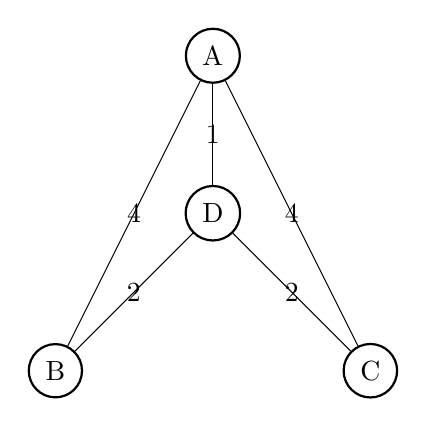
\begin{tikzpicture}
            \begin{scope}[every node/.style={circle,thick,draw}]
                \node (A) at (2,4) {A};
                \node (B) at (0,0) {B};
                \node (C) at (4,0) {C};
                \node (D) at (2,2) {D};
            \end{scope}

            \begin{scope}
                \path (A) edge node {$4$} (B);
                \path (A) edge node {$4$} (C);
                \path (A) edge node {$1$} (D);
                \path (B) edge node {$2$} (D);
                \path (C) edge node {$2$} (D);
            \end{scope}
            \end{tikzpicture}
        \end{center}
        There is only one MST $T = \{ (D,A), (D,B), (D,C)\}$ for $G$ with $w(T) = 4$. There is only one MST $T' = \{(A,C), (A,B), (D,A) \}$ given fixed leaves $L$ for $G$ with $w(T) = 9$. Note $T\neq T'$ and $w(T) < w(T')$. 
        \begin{enumerate}
            \item The existence of $T$, a MST of $G$ but not the a solution to MST with fixed leaves problem, disproves this claim 
            \item The existence of $T'$, a MST of $G$ with fixed leaves problem but not an MST for $G$, disproves this claim
        \end{enumerate}
        
    \end{solution}
    \item Write a greedy algorithm to solve the MST with Fixed Leaves problem. Give a detailed pseudo-code implementation of your algorithm, as well as a high-level English description of the main steps in your algorithm. What is the worst-case running time of your algorithm? Justify briefly.


    \textbf{Algorithm}
    \begin{enumerate}
        \item Let $S = V \setminus L$
        \item Find MST for graph induced by $S$, let $T_S$ be the ouput MST for $S$
        \item For each $(u,v)$ where $u\in L$ and $v\in S$, adds the lowest weight edge for each $u$ to $T_S$. In other words, find the light edge crossing the cut $(\{u \}, T_S)$ and adds it to $T_S$
        \item Return the augmented $T$, consists of $T_S$ and edges added to it in the previous step
    \end{enumerate}
    \textbf{Analysis}
    \begin{enumerate}
        \item Assume sets $S$ and $T$ membership check can be done in $O(1)$ time, this is possible if keep an extra bit in adjacency list representation of the graph. Assume insertion to array $T$ takes $O(1)$ time.
        \item $\textsc{MST-Kruskal}$ has worst case running time of $O(E\lg V)$
        \item The for loop executes $O(E)$ times altogether, since sum of lengths of all adjacency list is $2|E|$ for undirected graphs and $|L| \leq |V|$. In each iteration, membership check and potential assignment operation takes $O(1)$. 
        \item The entire algorithm has a worst time running time of $O(E\lg V)$
    \end{enumerate}


    \begin{algorithm}[H]
        \SetKwFunction{mst}{Find-MST-Fixed-Leaves}
        \SetKwFunction{kruskal}{MST-Kruskal}


        \Fn{\mst$(G,w,L)$}{
            $S \leftarrow V \setminus L $\\
            $G' \leftarrow $ induced by $S$\\
            $T  \leftarrow \kruskal(G',w)$\\
            \For{$u\in L$}{
                $e_{light} \leftarrow Nil$\\
                $w_{light} \leftarrow \infty$\\
                \For{$v\in G.Adj[u]$}{
                    \If{$v \in S$ and $w(u,v) < w_{light}$}{
                        $w_{light} \leftarrow w(u,v)$\\
                        $e_{light} \leftarrow (u,v)$
                    }
                }
                $T \leftarrow T \cup \{ e_{light}\}$
            }
            \Return{$T$}
        }
    \end{algorithm}

    \item Write a detailed proof that your algorithm always produces an optimal solution.


    \begin{lemma*}
        Given condition provided by the algorithm, provided that there is a valid solution for fixed leaves problem, then for any $u\in L$, there exists some $v\in S = V\setminus L$ such that $(u,v) \in E$. 
        \begin{proof}
            Prove by contradiciton. Assume there exists $u\in L$ such that for all $(u,v)\in E'= E$, we have $v\in L$. Pick any appropriate edge $(u,v)\in E'$ to be in some valid solution MST $T$. Now vertex $u$ and $v$ has one edge incident on it. We cannot include any other edge such that they incident on $u$ or $v$ since otherwise $u$ or $v$ would not be leaves (i.e. have degree of more than 1). Therefore $\{ u,v\}$ is isolated from the rest of the vertices, hence no viable MST exists possibly as a solution. Since we are given there is some solution to the problem, the claim thus holds
        \end{proof}
        
    \end{lemma*}



    \begin{proposition*}
        Given $G = (V,E)$ with cost function $c: E\to\R$ and a subset $L\subseteq V$, the algorithm returns MST $T$ where every $u\in L$ is a leaf and $T$ has the minimum cost amongst such spanning trees

        \begin{proof}
            By correctness of Kruskal's algorithm, \textsc{MST-Kruskal} terminates and returns $T_S$, which is a MST for $S = V\setminus L$.
            \begin{enumerate}
                \item Prove every $u\in L$ is a leaf in $T$. The algorithm finds and adds the least weight edge connecting $u$ to some $v\in S$. Since $T_S$ spans $S$ and the fact that the previous lemma holds, such operation is always possible. Since the algorithm only adds one, specifically $e_{light}$, to $T$ for each $u\in L$, $u$ has degree of one, hence are leaves in MST $T$
                \item Prove by contradiction that the algorithm returns a MST amongst such spanning trees. Assume there is some other spanning tree $T'$ such that $w(T) > w(T')$. We can decompose $T' = T_S' \cup T_O'$ where $T_S'$ is a subset of $T'$ and spans $S$ and $T_O'$ be the rest of edges in $T'$, specifically $T_O'$ consists of edges that crosses the cut $(L, S)$. 
                \begin{enumerate}
                    \item By correctness of \textsc{MST-Kruskal} we have 
                    \[
                        w(T_S) \leq w(T_S')
                    \]
                    \item After finding $T_S$, the algorithm then construct the solution MST $T$ by adding $(u,v)$ to $T_S$ where $v\in S$ for each $u\in L$ (Note this is always possible with previous lemma) such that $w(u,v)$ is minimized. Denote $E'$ be such set of edges added to $T_S$
                    Therefore  
                    \[
                        \sum_{e \in E'} w(e) \leq w(T_O')
                    \]
                \end{enumerate} 
                Althgether we have 
                \[
                    w(T) = w(T_S) + \sum_{e \in E'} w(e) \leq w(T_S') + w(T_O') = w(T')
                \]
                which contradicts the assumption that $w(T) > w(T')$. Therefore the claim holds
            \end{enumerate}
            This completes the proof
        \end{proof}
    \end{proposition*}


\end{enumerate}
    

\subsection*{Problem 3}


An edge in a flow network is called critical if decreasing the capacity of this edge reduces the maximum possible flow in the network. Give an efficient algorithm that finds a critical edge in a network. Give a rigorous argument that your algorithm is correct and analyse its running time.

\begin{solution}

    \textbf{Algorithm}
    \begin{enumerate}
        \item Find a maximum flow $f$ for $G$, let $G_f$ be the residual flow network for $G$ given $f$
        \item Return the set of edges $E' \subseteq E$ for which $f(u,v) = c(u,v)$, $(u,v) \in E'$
    \end{enumerate}
    \textbf{Analysis}
    \begin{enumerate}
        \item \textsc{Ford-Fulkerson} runs in $O(VE)$
        \item The for loop iterates $|E|$ times, doing a constant $O(1)$ operation to update $E'$. Suppose $E"$ is implemented with an array, the operation to insert an element at the end takes $O(1)$ time. Therefore the loop has a worst time running time of $O(E)$
        \item Altogether the algorithm has a worst case running time of $O(VE)$ 
    \end{enumerate}

    \begin{algorithm}[H]
        \SetKwFunction{crt}{Find-Critical-Edge}
        \SetKwFunction{ff}{Ford-Fulkerson}
        
        \Fn{\crt$(G, s, t)$}{
            $f \leftarrow \ff(G, s, t)$\\
            $E' \leftarrow \emptyset$\\
            \For{$(u,v)\in G.E$}{
                \If{$f(u,v) = c(u,v)$}{
                    $E' \leftarrow E' \cup \{ (u,v)\}$
                }
            }
            \Return{$E'$}
        }
    \end{algorithm}


    \textbf{Proof of Correctness}

    \begin{lemma*}
        Given a maximum flow $f$ for flow network $G$ and its residual flow network $G_f$. If any $(u,v)\in E$ such that $f(u,v) = c(u,v)$, then $(u,v)$ is in the cut-set of some cut $C = (S,T)$, where $s\in S$, $t\in T$, and such that $|f| = c(S,T)$.
        \begin{proof}
            Prove by contradiction. Assume there is no such cut $C$ where $(u,v)$ crosses $|f| = c(S,T)$. Then it must be that for all cut $C' = (S', T')$ that $(u,v)$ crosses, $|f| < c(S,T)$ by the upper-bound property, therefore
            \[
                |f| = f(S', T') = \sum_{u\in S'} \sum_{v\in T'} f(u, v) - \sum_{u\in S'} \sum_{v\in T'} f(v, u)   < c(S,T) = \sum_{u\in S'} \sum_{v\in T'} c(u, v) 
            \]
            This implies that there is some other edge $(x,y)$ in the cut-set of $C'$ such that $f(x,y) < c(x,y)$. Since $C'$ is an arbitrary and the above claim holds for all cuts, we can construct an augmenting path $p = \langle v_0, \cdots, v_k \rangle$ in $G_f$ by picking appropriate cuts such that $f(v_{i-1}, v_i) > 0$ for all $i = 1,\cdots, k$. This contradicts with the assumption that the algorithm for finding max flow terminates, specifically when there is no augmenting paths left. Hence the claim holds.
        \end{proof}
    \end{lemma*}

    \begin{proposition*}
        Given a maximum flow $f$ for flow network $G$ and its residual flow network $G_f$. the set of edges $E' \subseteq E$ for which $f(u,v) = c(u,v)$, $(u,v) \in E'$ is the set of critical edges
        \begin{proof}
            Given assumption of the proposition and previous lemma, we have $(u,v)$ in some cut $C =(S,T)$ such that $|f| = c(S,T)$. Since algorithm for finding the max flow $f$ terminates, by the max-flow min-cut theorem, the cut $C$ has minimal capacity, which bounds the value of the flow $|f|$. Hence, a reduction in $c(u,v)$ causes reduction in $C(S,T)$, and ultimately the maximum value a flow can achieve. Therefore $(u,v)$ is a critical edge. Since $(u,v)$ is an arbitrary edge in $E'$, $E'$ is the set of critical edges. 
        \end{proof}
    \end{proposition*}

\end{solution}


\subsection*{Problem 4}

\begin{enumerate}
    \item Suppose we want to compute the shortest path from node $s$ to node $t$ in a directed graph $G=(V,E)$ with edge lengths $l_e >0$ (assume integer valued lengths) for each $e\in E$. Show that this is equivalent to finding a pseudo-flow $f$ from $s$ to $t$ in $G$ such that $|f | = 1$ and $\sum_{e\in E} l_e f_e$ is minimized. There are no capacity constraints. Part of this problem requires you to define precisely what we mean by “pseudo-flow” in a general, directed graph. This is a natural extension of the notion of flow in a network.

    \begin{solution}
        Define a pseudo-flow as a function $f: V\times V \to \R$ such that $f_{uv}$ represents units of flow from vertex $u$ to $v$. $f$ still satisfies flow conservation but there is no capacity constraints on the amount of units of flow sent through the network. Given 
        \[
            |f| = \sum_{v\in V} f_{sv} = 1
        \]
        we require exactly one unit of flow from the source, and since the graph is connected and by flow conservation, this one unit of flow is tranferred conceptually from $s$ to $t$ over vertices in some arbitrary path $p = \langle v_0 = s,v_1, \cdots, v_k = t\rangle$ such that $f_{v_{i-1}v_i} = 1$ for all $i = 1,\cdots, k$. We claim that  
        \begin{center}
            there is not a flow $f_{uv} > 0$ such that $(u,v)$ is not in $p$. 
        \end{center}
        Prove by contradiction, if there is such a flow $f_{uv} = 1$ for $u\to v$ where $(u,v)$ is not in $p$, then to satisfy flow conservation, there must be some paths $p_1$ $p_2$ such that 
        \[
            p' = s \overset{p_1}{\leadsto} u \to v \overset{p_2}{\leadsto} t
        \]
        Since $(u,v)$ is not in $p$ by assumption, then $p' \neq p$, we then have 2 paths originated from $s$, with $|f| = 2$, then all $(u,v)$ with positive flow $f_{uv} > 0$ is in path $p$. Therefore,
        \[
            \sum_{e\in E}l_e f_e = \sum_{e \text{ in } p} l_e \times 1 + \sum_{e\text{ not in } p} l_e \times 0 = \sum_{e \text{ in } p} l_e = w(p)
        \]
        Minimizing $\sum_{e\in E}l_e f_e$ is equivalent to minimizing $w(p)$. Hence, the procedure of finding a pseudo-flow $f$ from $s$ to $t$ such that $|f| = 1$ and $\sum_{e\in E} l_e f_e$ is minimized is equivalent to finding a path $p$ with minimum weight $w(p)$, which is what shortest-path specifies 
    \end{solution}
    \item Write the shortest path problem as a linear or integer program where your objective function is minimized, based on your answer to the previous part. Give a detailed justification that your solution is correct.
    \begin{solution}
        \begin{align*}
            \textbf{Minimize:}\quad & \sum_{e\in E}l_e f_e \\
            \textbf{Subject to:}\quad & \sum_{v\in V} f_{uv} - \sum_{v\in V} f_{vu} = 
                                      \begin{cases}
                                          1 & \text{if } u = s\\
                                          -1 & \text{if } u = t \\
                                          0 & \text{otherwise}  \\
                                      \end{cases}\\
                                \quad & f_e \geq 0 \quad \text{for all } e\in E\\
        \end{align*}
        The linear program is basically a formal specification of the assumptions made for finding pseudo-flow $f$ from $s$ to $t$ in $G$. Since if $u=s$ we have 
        \[
            \sum_{v\in V} f_{sv} - \sum_{v\in V} f_{vs} = |f| = 1
        \]
        as well as flow conservation given by
        \[
            \sum_{v\in V} f_{uv} - \sum_{v\in V} f_{vu} = 0 \quad \iff \quad  \sum_{v\in V} f_{uv} = \sum_{v\in V} f_{vu}
        \]
        for all $u,v\in V\setminus \{ s,t\}$. Note a feasible solution is simply values $f_e$ for all $e\in E$, in other words, a function $f:V\times V\to\R$. Since flow conservation property is satisfied, this is saying that we are trying to find the pseudo-flow $f$ such that $|f| = 1$ and $\sum_{e\in E}l_e f_e$ is minimized. This is equivalent to finding the solution to shortest path problem as justified in the previous question. Now we prove linear program yields correct solution. Let $f$ be solution to the linear program. Let $p$ be the path such that for all edges $e$ in $p$, we have $f_e = 1$. Such path is always possible by the fact that we constrain source to admit 1 unit of flow and sink to accept 1 unit of flow. Now we prove that the path is the shortest. Prove by contradiction, assume there is some other path $p'$ with
        \[
            w(p') < w(p) = \sum_{e \text{ in } p} l_e = \sum_{e \text{ in } p} l_e \times 1 + \sum_{e\text{ not in } p} l_e \times 0 = \sum_{e\in E}l_e f_e
        \] 
        which contradicts the fact that $\sum_{e\in E}l_e f_e$ is minimal. Hence the solution to linear programming is correct. Note the transformation in the equation is possible as proved in the previous question
    \end{solution}

\end{enumerate}



\subsection*{Problem 5}

\begin{enumerate}
    \item In the Traveling Salesman Problem (TSP), we are given a directed graph $G = (V,E)$ with an integer weight $w(e)$ for each edge $e \in E$, and we are asked to find a simple cycle (more strict than MST, since MST cannot have cycle) over all the vertices (a “circuit”) with minimum total weight. (Note that the weights $w(e)$ can be positive or negative.) Show how to represent an arbitrary instance of the TSP as an integer program. Justify that your representation is correct, and describe how to obtain a solution to the instance of the TSP from solutions to your integer program.

    \begin{solution}
        We formulate similarly to problem 4. Pick arbitrary $s\in V$, add another vertex $t$ and its incident edges to $G$ such that $t$ has the exact same incident edges (including their weights) of $s$. Let $G' = (E', V')$ be the resulting graph. Consider pseudo-flow $f:V\times V \to \R$ be units of flow from $s$ to $t$. the value of $f_e$ determines if an edge is used in the circuit.
        \begin{align*}
            \textbf{Miminize: }\quad & \sum_{e\in E'} w(e)f_e \\
            \textbf{Subject to: } \quad & \sum_{v\in V'} f_{uv} - \sum_{v\in V'} f_{vu} = 
                                                    \begin{cases}
                                                        1 & \text{if } u = s\\
                                                        -1 & \text{if } u = t\\
                                                        0 & \text{otherwise }\\
                                                    \end{cases}\\
                                \quad & \sum_{v\in V'} f_{uv} = 2 \quad \text{for all } u\in V' \setminus \{ s,t\} \\
                                \quad & f_e \geq 0 \quad \text{for all } e\in E\\
        \end{align*}
        The first constraint given states that the model follows flow conservation and that the demand is 1 unit of flow. The second constraint states that any vertex has 2 incident edges for which the flow go through, therefore any edge in $E' \setminus \{s,t \}$ has degree 2. Altogether the feasible region consists of a flow $f$ such that for all $(u,v)\in E'$ for which $f_{uv}\neq 0$ forms a simple path from $s$ to $t$. The path is simple and spanning precisely because every vertex except from start and end has degree 2. Since we are minimizing $\sum_{e\in E'} w(e)f_e$, the path will be least weight. Therefore, if LP has a solution, the resulting $f_e$ specifies the least weight flow from $s$ to $t$. Let $E_p \subseteq E'$ be a set of edges where $f_e = 1$ for all $e\in E_p$. Now to get the simple cycle, we first replace the instance of vertex $t$ with $s$ in edges in $E'$, then start from $s$, and add $u$ to the sequence of vertices if $(s,u) \in E_p$. 
    \end{solution}

    \item  Your company has recently discovered that several of its problems can be solved using linear programming. Your company doesn’t want to write their own solver program, since many efficient programs are available for sale. But your boss has been reading his spam again and went out and purchased the MELPSE system (Most Efficient Linear Program Solver Ever!) in a fit of misdirected leadership. As expected, the claim is slightly overstated, and the package comes with some serious limita- tions. From the advertisement:

    \begin{center}
        MELPSE is the fastest and most streamlined LP solver ever! Using the latest technology, it will find the best non-negative values for all your variables, get the biggest value for your objective function, and it will even make sure that $Ax\leq b$!
    \end{center}

    In fact, this is all that MELPSE can do: it only supports non-negative variables (it implicitly enforces a constraint $x_1\geq 0$ on all variables $x_i$ ), only allows maximizations of the linear objective function, and insists that all constraints are in the form  $\sum_{i=1}^n a_{j,i} x_i \leq bj$ (where $a_{j,i}$ and $b_j$ are real numbers, perhaps negative). \\
    The linear programs you need to solve are usually minimization problems, where variables occasionally take negative values, and some constraints are expressed with equality or greater- than-or-equal. The boss has already spent your entire budget, so to save your team you will need to figure out how to use the MELPSE system to solve your problems.
    \begin{enumerate}
        \item One of your problems fits the restrictions of MELPSE except that you need to minimize your objective function. Describe precisely how to convert your program into one MELPSE can solve; that is, describe how to create an equivalent LP where the objective is being maximized. Briefly explain how to use a solution to your new program to find a solution to your original problem. 
        \begin{solution}
            Given a minimization linear program $L$, we can convert $L$ to an equivalent maximization linear program $L'$ by negating the coefficients in the objective function. $L$ and $L'$ are equivalent since they share the same feasible solution (since constraints unchanged) and for each feasible solution, the objective value in $L$ is the negative of the objective value in $L'$, therefore by definition of equivalence, $L$ and $L'$ are equivalent. The solution to the converted $L'$ is the solution to $L$ without any modification
        \end{solution}
        \item Another of your problems contains a constaint of the form $a_1 x_1 + a_2 x_2 + \cdots + a_x x_n \geq b$ Describe precisely how to convert this to a constraint of the form $a_1' x_1 + a_2' x_2 + \cdots + a_x' x_n \leq b'$ as required by MELPSE.
        \begin{solution}
            Let $a_i' = -a_i$ for all $i = 1, \cdots, n$ and let $b' = -b$
        \end{solution}
        \item This problem also has a constraint of the form
        \[
            a_1 x_1 + a_2 x_2 + \cdots + a_x x_n = b
        \]
        Describe precisely how to create an equivalent LP that can be solved by MELPSE (or in the form of part (b)).
        \begin{solution}
            Replace the given equality constraint with 
            \[
                a_1 x_1 + a_2 x_2 + \cdots + a_x x_n \leq b \quad \text{ and } \quad a_1 x_1 + a_2 x_2 + \cdots + a_x x_n \geq b
            \]
            The resulting LP are equivalent because the objective function is unchanged and the constraints are equivalent because of the fact that 
            \[
                a = b \iff a \geq b \land a \leq b
            \]
        \end{solution}
        \item From the previous parts we know how to solve a minimization problem with $\geq$ or $=$
        constraints. We can assume that all constraints are in the form $a_1x_1 + a_2x_2 + \cdots + a_nx_n \leq b$. But we have a problem where one of the variables, $x_1$, could be negative. Describe precisely how to construct an equivalent LP where we replace $x_1$ with two new variables which can only take non-negative values. Briefly explain how to use a solution to your new program to find a solution to your original problem.
        \begin{solution}
            Replace each occurrence of $x_1$ in original LP $L$ with $x_1' - x_1''$ in both the objective function and the constraints, add the constraints $x_1', x_1'' \geq 0$. let $L'$ be the resulting LP. A feasible solution $\hat{x}$ to $L'$ corresponds to a feasible solution $\bar{x}$ to $L$ where $\bar{x}_1 = \hat{x}_1' - \hat{x}_1''$. Conversely, a feasible solution $\bar{x}$ to $L$ corresponds to a feasible solution $\hat{x}$ given by 
            \begin{enumerate}
                \item $\hat{x}_1' = \bar{x}_1$ and $\hat{x}_1'' = 0$ if $\bar{x}_1 \geq 0$. 
                \item $\hat{x}_1' = 0$ and $\hat{x}_1'' = \bar{x}_1$ if $\bar{x}_1 < 0$.
            \end{enumerate}
            Therefore, $L$ and $L'$ are equivalent. Note the above 2 points are always the case because $x_1'$ and $x_1''$ are always of different signs. And if both are in the objective function, the positively signed variable will be optimized in the objective function, to the point such that the other variable is 0.
        \end{solution}
        \item Write an efficient high-level algorithm that will convert a linear program that might be a maximization problem, might contain greater-than-or-equal or equality constraints, and may contain variables lacking a non-negativity constraint, into an equivalent linear program that can be solved by MELPSE. Give a good bound on the size (the size being the number of variables and number of constraints) of your new linear program and briefly justify it.
        \begin{solution}
            \textbf{Algorithm}
            Let $L' = (A', b', c')$ be the result given $L = (A, b, c)$. Let there be $n$ variables in the solution and $m$ constraints
            \begin{enumerate}
                \item If the algorithm is as minimization linear program, let $c' = -c$
                \item If there exists a constraint $\sum_{j=1}^n a_{ij} x_j = b_i$ for some $i = 1,\cdots, m$, replace the constriant with $\sum_{j=1}^n a_{ij} x_j \geq b_i$ and $\sum_{j=1}^n a_{ij} x_j \leq b_i$
                \item If there exists a constraint  $\sum_{j=1}^n a_{ij} x_j \geq b_i$ for some $i = 1,\cdots, m$,  let $a_{ij}' = -a_{ij}$ for all $j = 1,\cdots, n$, and revert the sign from $\geq$ to $\leq$
                \item if exists a negative variable $x_j < 0$ for some $j=  1,\cdots, n$, then replace $x_j$ with $x_j' - x_j''$ in LP and add constraints $x_j', x_j'' \geq 0$
            \end{enumerate}
            Now we discuss worst case size of the resulting $L'$. The worst case happens when we have an unconstrained $x_j$ for all $j = 1,\cdots, n$ variables and that every constaint is an equality constraint. 
            \begin{enumerate}
                \item For each $x_j$ lacking a nonnegative constraint, the conversion doubles the size of variables by removing one variable $x_j$ and adding 2 variables $x_j', x_j''$ into $L'$. Hence size of variable at most doubles. The conversion also introduces $2n$ nonnegative constraints for $x_j'$ and $x_j''$
                \item For each equality constraint, the conversion replaces the constraint with 2 inequality constraints, therefore the size of constraint at most doubles
            \end{enumerate}
            Altogether, the size of $L'$ is bounded by $2n + 2n + 2m = 4n + 2m$
        \end{solution}
    \end{enumerate}

\end{enumerate}





\end{document}
